\documentclass{amsbook}
\usepackage{graphicx} % Required for inserting images
\usepackage{float}
\usepackage[colorlinks=true,linkcolor=blue]{hyperref}
\usepackage{amssymb}
\usepackage{enumerate}
\usepackage{mathtools}
\usepackage{tikz}
\usepackage[answerdelayed]{exercise}
\usepackage{floatflt}
\usepackage{multicol}
\usepackage{subcaption}
\usepackage{tikz}
\usepackage{tkz-euclide}
\usetikzlibrary{trees}

\usepackage[backend=biber,style=alphabetic,sorting=ynt]{biblatex}
\addbibresource{calc.bib}

\setlength{\parindent}{0pt}
\setlength{\listparindent}{0pt}
\renewcommand{\ExerciseHeaderTitle}{\quad\ExerciseTitle}
\renewcommand{\AnswerHeader}{\medskip\centerline{\emph{\ExerciseName\ \ExerciseHeaderNB} \smallskip}}
\renewcommand{\ExerciseHeader}{\medskip\ExerciseHeaderDifficulty{\emph{\ExerciseName\ \ExerciseHeaderNB\ExerciseHeaderTitle} \newline}}
\renewcommand{\QuestionNB}{(\alph{Question})\ }
\renewcommand{\Re}{\operatorname{Re}}
\renewcommand{\Im}{\operatorname{Im}}


%%%%%%%%%%

\begin{document}

\title{Calculus Problem Book:\\
    \Large Form V and Form VI}


\author{S. Chu}

\maketitle
\tableofcontents
\chapter*{Preface}
The following short booklet contains a collection of problems with solutions that roughly follow the topics typically covered in the calculus sequence for Form V and Form VI mathematics classes at Ethical Culture Fieldston School. The hope is to provide a book of problems of varying difficulty that will provide non-routine exercises as well as to record general themes and approaches to tackling these types of problems in general. Ideally these problems can be useful to all courses that cover these topics. Problems are roughly categorized by difficulty level and notated via *, **, or *** in increasing difficulty. We have adopted problems from memory, and from years of working with the material. The following references were consulted for problems as well as other considerations such as narrative structure in introducing various topics and thematic development of the material. \cite{mcirc}, \cite{aops}, \cite{hpn}, [more later].
\chapter{Functions and Other Miscellaneous Content}

\section{Set Notation and Numbers}
\begin{Exercise}[title={Sets, Unions and Intersections}, difficulty = 0, label= 1b1]
	Set $A \subset B$ iff every element of $A$ in also in $B$. Set $A \supset B$ iff every element of $B$ is also in $A$ and two sets are equal iff both $A\supset B$ and $A\subset B$. 
	\begin{enumerate}
		\item If $A \subset B$ then what is the set $A \cap B$?\\
		\item If $A \subset B$ then what is the set $A \cup B$?\\
		\item If $A \cup B = B$, give an argument that explains why $A \subset B$.
	\end{enumerate}
	
\end{Exercise}

\begin{Exercise}[title={Complements}, difficulty=0, label = 1b2]
	Given a set $A$, and a set $B$ we can define the complement of that set, $A^c$ or sometimes: $\overline{A}$, $A'$, or $B-A$, as the elements in $B$ but not in $A$.  Notice $A^c, A'$ and $\overline{A}$ do not reference the set $B$ and are often used when no confusion can arise or there is some all encompassing universal set $U$ that contains $A$.
		\begin{enumerate}
			\item Given a universal set $U$ and $A, B$ contained in $U$. Show that $ (A\cap B)^c =A^c \cup B^c$ by first showing that $(A \cap B)^c \subset A^c \cup B^c$. Then show that $(A \cap B)^c \supset A^c \cup B^c$. This property is often called DeMorgan's Law.
			\item Describe the elements that are contained in the set $(A-B) \cup (B-A)$. This set is called the symmetric difference of A and B, or $A \Delta B$.
		\end{enumerate}

\end{Exercise}

\begin{Exercise}[title={Working with Sets}, difficulty=2, label=1b3]

	In the previous problem we defined the symmetric difference. The following exercises will work through some properties of this operation on sets. Recall that to show two sets $A, B$ are equal you must show that $A \subset B$ ie. every element is $A$ is also in $B$, as well as that $B \subset A$, ie. every element of $B$ is also in $A$.
	\begin{enumerate}
		\item Show that $(A-B) \cup (B-A) = (A \cup B) - (A\cap B)$ as sets. These are two different ways to think about the set that is the symmetric difference of two sets $A \Delta B$. Let $A, B$ be arbitrary sets.
		\item Show that $A \Delta B = B \Delta A$ by showing that every element in the set on the left is in the set on the right and vice versa.
		\item Show that $A \Delta \varnothing  = A$. Where $\varnothing$ is the empty set.
		\item Show that $A \Delta A = \varnothing$.
		
		
	\end{enumerate}

\end{Exercise}

%%%%
%%%%

\section{Working with Inequalities}

%%%%
%%%%

\section{Polynomials}


%%

\begin{Exercise}[title={Polynomials I}, difficulty=0 , label=1a1 ]
	Let $f(x)=x^2-3$ and $g(x)=x^3-2x$. Both $f$ and $g$ are polynomials. You can form new polynomials by adding, subtracting, multiplying, and composing. 
        \begin{enumerate}
            \item Find $(f+g)(x)$
            \item Find $(f-2g)(x)$
            \item Find $(f\cdot g)(x)$
            \item Find $f \circ g)(x)$
            \item Explain why $(f/g)(x)$ is not a polynomial.
        \end{enumerate}

	\hfill \emph{solution} \refAnswer{1a1}
\end{Exercise}

\begin{Answer}[ref={1a1}]
	blah blah
\end{Answer}

\begin{Exercise}[title={Defining Polynomials}, difficulty=1, label=1a2]
A polynomial $f$ has the general form $f(x)=a_0+a_1 x + a_2 x^2 + \ldots +a_{n-1}x^{n-1} + a_nx^n$, where $n \in \mathbb{Z}$ and $a_i \in \mathbb{R}$. Show that adding, subtracting, or multiplying two polynomials always results in a polynomial. Explain why this is not the case for division.

    \hfill \emph{solution} \refAnswer{1a2}
\end{Exercise}

\begin{Answer}[ref={1a2}]
    The expression $A \subset B$ is read, the set $A$ is contained in the set $B$. Whereas the expression $A \supset B$ is read the set $A$ contains the set $B$.
    \begin{enumerate}
        \item $\mathbb{Z}\supset \mathbb{N}$
        \item $\mathbb{R}\supset \mathbb{Q}$
        \item $\mathbb{N} \subset \mathbb{Q}$
    \end{enumerate}
\end{Answer}

\begin{Exercise}[title={Polynomials II}, difficulty =0, label=1a3]
   A function $f$ is even if and only if $f(x)=f(-x)$ for all $x$ in its domain. A function is odd if and only if $f(-x)= - f(x)$ for all $x$ in its domain.
   	\begin{enumerate}
   		\item Give an example of an even polynomial.
   		\item Give an example of an odd polynomial.
   	\end{enumerate}
\end{Exercise}

%%%%%%%%%%%%%%%%%%%%%%%%%%%%%%%%%%%%%%%%


\section{Trigonometric Functions}

%%%%%%

\section{Miscellaneous}

%%%%%%%%%%%%%%%%%%
%%%%%%%%%%%%%%%%%%
\chapter{Limits and Continuity}


\section{Intuitive Notion}

\section{Epsilon and Delta}

\begin{Exercise}[title={Dirichlet Function}, difficulty=1 , label=2b1 ]
	The Dirichlet function $D$ is define as $D(x)=\left\{\begin{array}{c l} 1 & x\in \mathbb{Q} \\ 0 & \mbox{otherwise}\end{array} \right.$. Two sets of numbers are \emph{not seperable} if it is impossible to find an open interval around an element from one set that contains only elements from that set and not the other. Rational numbers and irrational numbers are not separable. Use this  to argue that $\lim \limits_{x\to a} D(x)$ does not exist for any value of $a$.
	\hfill \emph{solution} \refAnswer{2b1}
\end{Exercise}

\begin{Answer}[ref={2c1}]
	blah blah
\end{Answer}
\section{Continuity}
\begin{Exercise}[title={A Bounded Function around Zero}, difficulty=1 , label=2c1 ]
	Let $f: \mathbb{R} \to \mathbb{R}$ be a function such that $|f(x)| \leq |x| $ for all $x$ in the domain of $f$.  Prove that $f$ is continuous at $x=0$.

	\hfill \emph{solution} \refAnswer{2c1}
\end{Exercise}

\begin{Answer}[ref={2c1}]
	blah blah
\end{Answer}

\begin{Exercise}[title={Some Points Don't Move That Much}, difficulty=1 , label=2c2 ]
	Let $f:[0,1] \to [0,1]$ be a function such that $|f(x)| \leq |x| $ for all $x$ in the domain of $f$.  Prove that $f$ is continuous at $x=0$.

	\hfill \emph{solution} \refAnswer{2c2}
\end{Exercise}

\begin{Answer}[ref={2c2}]
	blah blah
\end{Answer}


\section{Intermediate Value Theorem}
\begin{Exercise}[title={Degree 3 Polynomial with Real Roots}, difficulty=1, label=2d1]
Let $f(x)=(x-a)(x-b)+(x-b)(x-c)+(x-a)(x-c)$ where $a,b,c$ are distinct real numbers. Prove that $f$ must have 3 real distinct zeroes.


\end{Exercise}

\begin{Answer}[ref={2d1}]
	Look at $f(a)$, $f(b)$ and $f(c)$.  Since $a,b,$ and $c$ are distinct we can assume they are ordered $a<b<c$, this will then put you in a position to apply IVT.
\end{Answer}

\begin{Exercise}[title={Fixed points}, difficulty=1, label=2d2]
Let $f$ be a continous function from the unit interval to itself. $f:[0,1] \to [0,1]$. Show that $f$ must have at least one fixed point $x_0$.  In other words,  $f(x_0)=x_0$.

\end{Exercise}

\begin{Exercise}[title={Antipodes}, difficulty = 2, label=2d3]
Two points on a sphere are antipodal if the line connecting them passes through the center of the sphere. They are 'directly opposite' one another, or maximally distant from one another while still being on the sphere. 
	\begin{enumerate}
		\item If you assume that the earth is a sphere and that temperature varies continuously from point to point on the earth, show that there must be a pair of antipodal points that are the same temperature at a given moment in time.\\
		\item If we also assume that air pressure varies continuously across the earth, show that there must be a pair of antipodal points on the surface of the earth that have the same temperature and air pressure at a given moment in time. \\
	\end{enumerate}

\end{Exercise}

\begin{Answer}[ref={2d3}]
	Both require looking at the difference in the function evaluated at a pair of antipodes.
\end{Answer}

%%%%%%%%%%%
%%%%%%%%%%5i

\chapter{The Derivative}

\section{Limit Definition and Properties of the Derivative}
\begin{Exercise}[title={Introducing a Discontinuity}, difficulty=0, label=3a1]
Let $f(x)=|x|$. Use the limit definition of the derivative to show that $f'(x)=\dfrac{|x|}{x}$. Show using the definition of continuity how the derivative 

\end{Exercise}

\begin{Answer}[ref={3a1}]
    
\end{Answer}

\section{Tangent Line Problem}

\section{Higher Order Derivatives}

\section{Power Rule and others}
\begin{Exercise}[title={Unit Circle and Sine}, difficulty=1 , label= 3d1]
	Let $P=(\cos \theta,\sin \theta)$. Use similar triangles to calculate an approximation for $\dfrac{\Delta y}{\Delta \theta}$ and explain how this shows what the derivative of $f(x)=\sin (x)$ is.  Do the same for $g(x)=\cos(x)$ by looking at $\dfrac{\Delta x}{\Delta \theta}$.
		\begin{figure}[H]
			\centering
			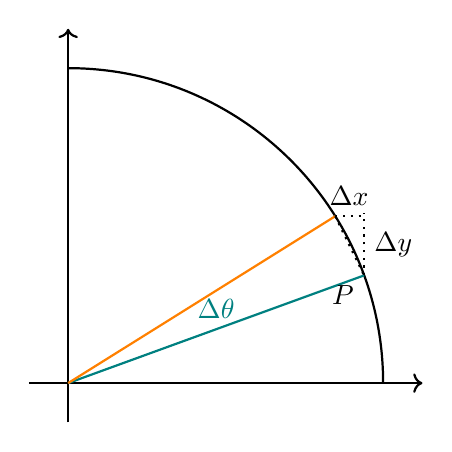
\begin{tikzpicture}
			\draw[thick](4,0)arc(0:90:4);
			\draw[thick,->](-.5,0)--(4.5,0);
			\draw[thick,->](0,-.5)--(0,4.5);
			\tkzDefPoint(4,0){A}
			\tkzDefPoint(0,0){B}
			\tkzDefPointBy[rotation=center B angle 20](A) \tkzGetPoint{C}
			\draw[thick, color=teal](B)--(C) node[midway, above]{$\Delta \theta$};
			\tkzDefPointBy[rotation=center B angle 12](C) \tkzGetPoint{D}
			\draw[thick, color= orange](B)--(D);
			\draw[thick,dotted](C)--+(0,.79) node[midway,right]{$\Delta y$};
			\draw[thick,dotted](D)--+(.35,0) node[midway, above]{$\Delta x$};
			\draw[thick,dotted](D)--(C) node[at end, below left]{$P$};
			\end{tikzpicture}
		\end{figure}

	\hfill \emph{solution} \refAnswer{3d1}
\end{Exercise}

\begin{Answer}[ref={3d1}]
	blah blah
\end{Answer}

\section{Implicit Differentiation}

%%%%%%%%%%
%%%%%%%%%%%

\chapter{Applications of the Derivative}

\section{Related Rates}

\section{Mean Value Theorem}

\section{Maximums and Minimums}

\section{Optimization and Graphing}

%%%%%%%%%
%%%%%%%%%

\chapter{The Integral}
\section{Series}

\section{Riemann Sums}


\section{Riemann Integrable}


\section{Properties of the Integral}


%%%%%%%%%%%
%%%%%%%%%%%%

\chapter{The Fundamental Theorem of Calculus}

\section{Anti-Derivatives}

\section{FTC part I}

\section{FTC part 2}

\section{Functions Defined by an Integral}

\section{Integral as Accumulator}

\section{U Substitution}

\section{Probability Distributions}

%%%%%%%%%%%%
%%%%%%%%%%%

\chapter{Logarithms, Exponentials, and Inverses}

\section{Logarithms}

\section{Inverse Functions}

\section{Exponentials}

\section{Inverse Trigonometric Functions}

\section{Hyperbolic Trigonometric Functions}



%%%%%%%%%%
%%%%%%%%%%%%

\chapter{Methods of Integration}


\section{Integration by Parts}

\section{Method of Partial Fractions}

\section{Trigonometric Substitutions}

\section{Improper Integrals}

%%%%%%%%%
%%%%%%%%%

\chapter{Differential Equations}
\section{Slope Fields and Euler's Method}

\section{Separation of Variables}

\section{Modeling}

\section{Logistic Growth}

\section{Systems of Differential Equations}

\section{Reduce 2nd order equations to two 1st order equations}


%%%%%%%%%%
%%%%%%%%%%

\chapter{More Applications of Integration}

%%%%%%%%%%
%%%%%%%%%%

\chapter{Infinite Series}

\chapter{Conics, Parametric Equations, Polar Coordinates}

\chapter{Vectors and the Geometry of $\mathbb{R}^3$}

\chapter{Vector Valued Functions}

\chapter{The Partial Derivative and Function of Several Variables}

\chapter{The Gradient and the Method of Lagrange Multipliers}

\chapter{The Derivative of maps from $\mathbb{R}^n \to \mathbb{R}^m$}

\chapter{Longer Problem Sets}
\newpage
    \section*{Working with Parameters and the Derivative}
    	In this exploration we will work with derivative to find tangent lines to a curve. We will also introduce working with parameters and see how this gives us a set of tools to solve more complex problems. We will end by using our skill with parameters to explore a little bit of the early history of Calculus by taking a look at Descartes' Method of Normals and Fermat's Method of Adequality.
    	\subsection*{First Let's Look at Tangent Lines to a Parabola}
    		\begin{enumerate}
    			\item Let $f(x)=x^2+1$ and point $C(0,-2)$. Find the equation of the two lines that pass through $C$ and are tangent to $f$.\\
    			
				\item Let $C$ vary its position along the $y$-axis. Let $C(0,k)$. Find the equations of the two lines that pass through $C$ and are tangent to $f$. Notice your solutions will be in terms of the 				parameter $k$.\\
				
				\item Lastly, let's generalize and let $C$ be any point in the plane $C(h,k)$. What are the equations of the two lines that pass through $C$ and are tangent to $f$, in terms of the parameters $h$ and $k$? \\
				\item Notice this gives you the equations for the lines through any point in the plane that are tangent to the given parabola. Demonstrate the ease with which you can find these lines that are tangent to the parabola, by finding them for $P(5,3)$ and $Q(3,-5)$.\\
				\item What do these equations tell you about the family of lines tangent to the graph of $f$? What points on the plane have no lines through them that are tangent to the curve? How can you see this from the equations? Explain how this is different than just looking at $f'(x)$?\\
    		\end{enumerate}
    		
    	\subsection*{Descartes' Method Of Normals versus Fermat's Method}
    	In this next section we will take a look at two early methods of finding slopes of lines tangent to a a curve.
    		
\newpage		
    \section*{An Algorithm to Find Roots}
   We will learn how to find the zeroes of a function $f(x)$ using Newton's Method, which involves using the derivative to find lines tangent to the curve and using these to successively better approximate the zeros of a function. 
    \begin{enumerate}
    	\item First recognize that finding the zero of a line is straightforward. We will reduce finding the zeroes of an arbitrary differentiable function to finding the zeroes of a bunch of lines. Let $y-a=m(x-b)$ be a line through $(b,a)$  with slope $m$. Find its $x$-intercept in terms of $a, b$ and $m$.\\
    	
    	\item We can get a sense for how the method works by looking at a quadratic $f(x)=-x^2+5x$.
    		\begin{enumerate}
    			\item First let's solve for the zeroes by factoring or using the quadratic formula. What are the zeroes of $f$?\\
    			\item Let's use the point $(4, 4)$ on $f$, and call our initial $x$ value  $x_0=4$. Find the line tangent to $f$ at $(4,4)$. Let's call this line $l_1$.\\
    			\item What is the $x$-intercept of $l_1$? Call the $x$-coordinate of the zero of $l_1$, $x_1$.\\
    			\item Notice $x_1$ is not equal to a zero of $f$, but it is closer than $x_0$. Let's repeat this process but using $(x_1,f(x_1))$.\\
    			\item What is the line tangent to $f$ at $(x_1,f(x_1))$? Find its $x$-intercept and call it $x_2$. It should be close to one of the zeroes at this point. \\
    			\item Give a sketch of each tangent line that you found in this problem and its $x$-intercept. Detail how this process works to approximate the zeroes of a function.\\
    			\item If your initial guess was $x_0=3$ Would the process converge to $x=5$ in more or fewer steps. Explain without carrying out the calcuations.\\
    			\item What initial guess would cause the process to fail? Explain why.\\
    		\end{enumerate}
    	\item The power of Newton's Method is that the same process can be applied to any differentiable function to find its zeroes.  One of its drawbacks is that it can involve a lot of calculation. Let's offload some of this to a spreadsheet, but first let's develop an expression to generate the sequence of $x$-coordinates, $\{x_0,x_1,x_2,\dots\}$ that should converge to the a zero of the given function.\\
    		\begin{enumerate}
    			\item Let $x_0$ be your first guess at a zero. Then as we saw before we are looking for the tangent line to $f(x)$ that passes through $x_0, f(x_0)$.  $x_1$ is the $x$-intercept of that tangent line. Find an expression for $x_1$ in terms of $x_0,f(x_0), and f'(x_0)$.  Generalize this to an expression that gives $x_n$.\\
    			\item Look at the spreadsheet linked here. 
    			\item Recall how difficult it is to find where the sine curve intersects with various lines. We will find when $y=2\sin(x)$ meets $y=x$ by letting $g(x)=2\sin(x)-x$ and solving for its zeroes. 
    			\item Use the IVT to get a guess for where $g(x)$ has zeroes. Then use \href{https://docs.google.com/spreadsheets/d/1FWjEk4M7XneAE1M9-i5LCKr_XWMnP2WlhSxLDb_xmX8/edit?usp=sharing}{the spreadsheet} to find these zeroes with a reasonabe first guess determined by your use of the IVT. Take a screen shot of your spreadsheet that shows the calculations that give each zero.
    			
    		
    		\end{enumerate}
    	
    \end{enumerate}
    
\newpage	
    \section{Instantaneous Rate of Turning}
    
    
\newpage	    
    \section*{Efficient Foraging}

\normalsize 
An Application of Optimization\footnote{adapted from Graves at NCSSM}
%specific topic
%%%%%%%
\\

%\emph{Complete all work on a separate sheet of paper with exercises clearly labeled and all reasoning and work given.}\\[.5cm]
%%\emph{Show all work for full credit.}
Foraging animals, whose food is arranged in clumps must make a decision about how long to stay in a given clump of food before moving on in search of another. We will try to arrive at an optimal strategy to foraging given a few simplifying assumptions. Let us first assume that patches of food are distributed uniformly (equally spaced) and that they are equally abundant, meaning an animal's optimal time spend in one patch would be the same for any other patch.
\begin{enumerate}
	
	\item Let us first try to model the rate at which resources can be gathered when arriving at a fresh patch.
		\begin{enumerate}
			\item What would a sketch of the amount of food gathered versus time look like assuming at time zero that no food had been gathered and the patch has a total of $L$ units of food?
			\item Explain why your sketch has the shape it has. What physical idea about the patch of food are you trying to capture? What criteria do you think would be common to all proposed models? Explain.
			\item Does the graph $F(t)=L(1-e^{-t/2})$ meet the criteria you gave in the previous question? Explain. Do you have a different function in mind? If so compare it to $F(t)$. What are its comparative strengths and weaknesses.
		\end{enumerate}
		\item Another factor to take into consideration is how long it takes to get from one patch of food to the next.
		\begin{enumerate}
			\item Let's look to extend our model from 1c by assuming it takes $A$ seconds to travel from each patch to a new patch, and that the closest patch to home is also $A$ seconds away. What does the graph of $F$ versus time look like for an animal that leaves home and forages in one patch? Give a labeled sketch.
			\item Give a piecewise defined function that will model the above situation. Use $f(t)=L(1-e^{-t/2})$ as the food gathering profile for one patch and $A$ as the time it takes to get to the patch.
			\item Sketch and give a piecewise defined function that will model $F$ versus time for an animal that leaves home and forages in two patches of food, where every patch is $A$ seconds away and the animal spends $B$ seconds in each patch. It may be easier to define $F(t)$ by using translates of $f(t)$.
		\end{enumerate}
		\item Let's take a moment to look at the various characteristics of our model so far.
			\begin{enumerate}
				\item What are some of the assumptions we are making in modeling this situation?
				\item The model gives energy gathered(F) in terms of time spent foraging (t). What are the three other factors or parameters that affect this model?
				\item Which of these parameters does the foraging animal have influence on?
				\item What is the same and what is different in the two following foraging strategies?\\
					\begin{figure}[H]
						\center
						\includegraphics[scale=.5]{b.png}
					\end{figure}
			\end{enumerate}
		\item Our main goal then is to model an animal's foraging behavior in choosing \underline{\hspace{4cm}} given a certain density of food patches (time between patches), and richness of food patches (ie.energy gathering profile of a patch) so that it will maximize the food it collects in a given time.
	\begin{enumerate}
		\item Here we have varied the density of the food patches while keeping each patch's food gathering profile the same. For which situation will the animal stay longer in one food patch? Why?
		\begin{figure}[H]
			\centering \includegraphics[scale=.55]{c.png}
		\end{figure}
		\item Here we have varied the food gathering profile of each patch, while keeping the density the same. For which situation will the animal stay onlger in one food patch? Why?
		\begin{figure}[H]
			\centering \includegraphics[scale=.55]{d.png}
		\end{figure}
	\end{enumerate}
\item Let's get more familiar with these ideas with some concrete models of bees foraging for pollen.
	\begin{enumerate}
		\item First, let's look at things graphically. Given the travel distance of 3 seconds and the food gathering profile given in the figure below, how much pollen is gathered over 12 seconds, if the bee stays on each flower 1 second versus 3 seconds. 
		\begin{figure}[H]
			\centering \includegraphics[scale=.75]{e.png}
		\end{figure}
	\item Assuming the food gathering profile is given by $f(t)=\sqrt{t}$, and a travel time of 3 seconds, let's look at the effect of various foraging times (time spent on a flower) on total collected pollen as well as average rate of pollen collected. Fill out the following table.\\[.5cm]
		\begin{tabular}{c|c|c|c}
			total time& foraging time& total pollen & avg rate of pollen collection\\
			\hline
			8 & 1 &&\\
			10 & 2 &&\\
			12 & 3 &&\\
			12 & 1 &&\\
			14 & 4 &&\\
			15 & 2 &&\\
			
		\end{tabular}
		\item Which foraging time seems optimal? Why?
	\end{enumerate}
	\newpage
	\item It may then be reasonable to assume that animals will choose the foraging time that maximizes the average rate of food gathering. Let $F(t)$ be one cycle of foraging that includes travel time $A$ with a food gathering profile $f(t)$.\\
	So $F(t)=\left\{ \begin{array}{c c l} 0 &,& 0\leq x < A\\ f(t-A) &,& A \leq x \end{array}\right.$
	\begin{enumerate}
	\item The average rate of food gathering is given by $G(t)=\dfrac{F(t)}{t}$. Assuming $t>0$, what equation must critical points of $G(t)$ satisfy? What does this look like on a graph of $F(t)$?
	\item Charnov in establishing the marginal value theorem says, "The predator should leave the patch it is presently in when the marginal capture rate in the patch drops to the average capture rate for the habitat." Explain how this is a restatement of what you found in the part a.
	\end{enumerate}
\item Determine the optimal foraging time $B$ for each of the following food gathering profiles and travel times.
	\begin{enumerate}
		\item $F(t)=\left\{ \begin{array}{c c l} 0 &,&0\leq t <3\\ \sqrt{t-3} &,& t\geq 3 \end{array}\right.$
		\item $F(t)=\left\{ \begin{array}{c c l} 0 &,& 0\leq t<A\\ K\sqrt{t-A} &,& t\geq A \end{array}\right.$
		\item $F(t)=\left\{ \begin{array}{c c l} 0 &,&0\leq t <3\\ \sqrt[3]{t-3} &,& t\geq 3 \end{array}\right.$
		\item $F(t)=\left\{ \begin{array}{c c l} 0 &,&0\leq t <A\\ \sqrt[n]{t-A} &,& t\geq A \end{array}\right.$
	\end{enumerate}
\item In the previous set of questions what do $n$, $A$, and $K$ represent in our foraging model, and how did changing these parameters affect the optimal foraging time? Explain.
\end{enumerate}

\newpage	    
    \section{When is Venus Bright in the Sky?}

\newpage	    
    \section{Rainbows}

\newpage	    
    \section{Constructing the Demand Curve}

\newpage	    
    \section{The Shape of Bee Hive Cells}

\newpage	    
    \section{The Art Gallery Problem}

\newpage	    
    \section{Getting to $\pi$ using Integration by Parts}

\newpage	    
    \section{Predicting Peak Oil}
    
\newpage	    
    \section{SIR: A Model for the Spread of Infectious Disease}

\newpage	    
    \section{Modeling Air Resistance}

\newpage	    
    \section{A Model for Combat}

\newpage	    
    \section{A Model for Relationships}

\newpage	    

%%%%%
%%%%%
%End of problems of the book.
%%%%%%%
%%%%%

\chapter{Answers}
\shipoutAnswer

\printbibliography
\end{document}
